\subsection{FHR Benchmark Specifications}
\begin{frame}
    \frametitle{FHR Benchmark Specifications}
    \begin{itemize}
        \item UIUC participates in the benchmark with OpenMC and using the ENDF/B-VII.1 material 
        cross section library
    \end{itemize}
    \vspace{-0.2cm}
    \begin{table}
        \caption{OECD NEA's FHR Benchmark Phases 
        \cite{petrovic_benchmark_2021}.}
        \vspace{-0.25cm}
        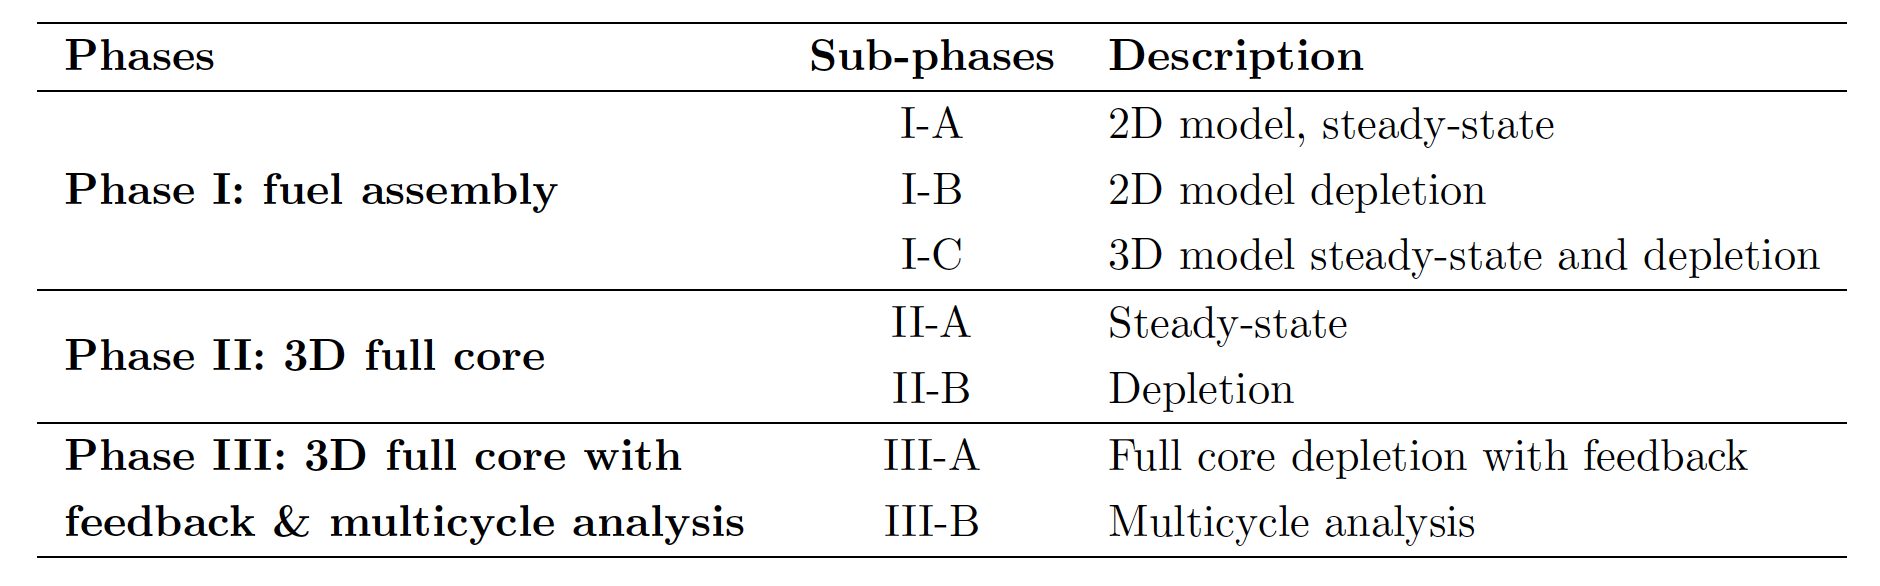
\includegraphics[width=0.7\linewidth]{figures/benchmark-phases.png} 
    \end{table}
    \vspace{-0.3cm}
    \begin{figure}[]
        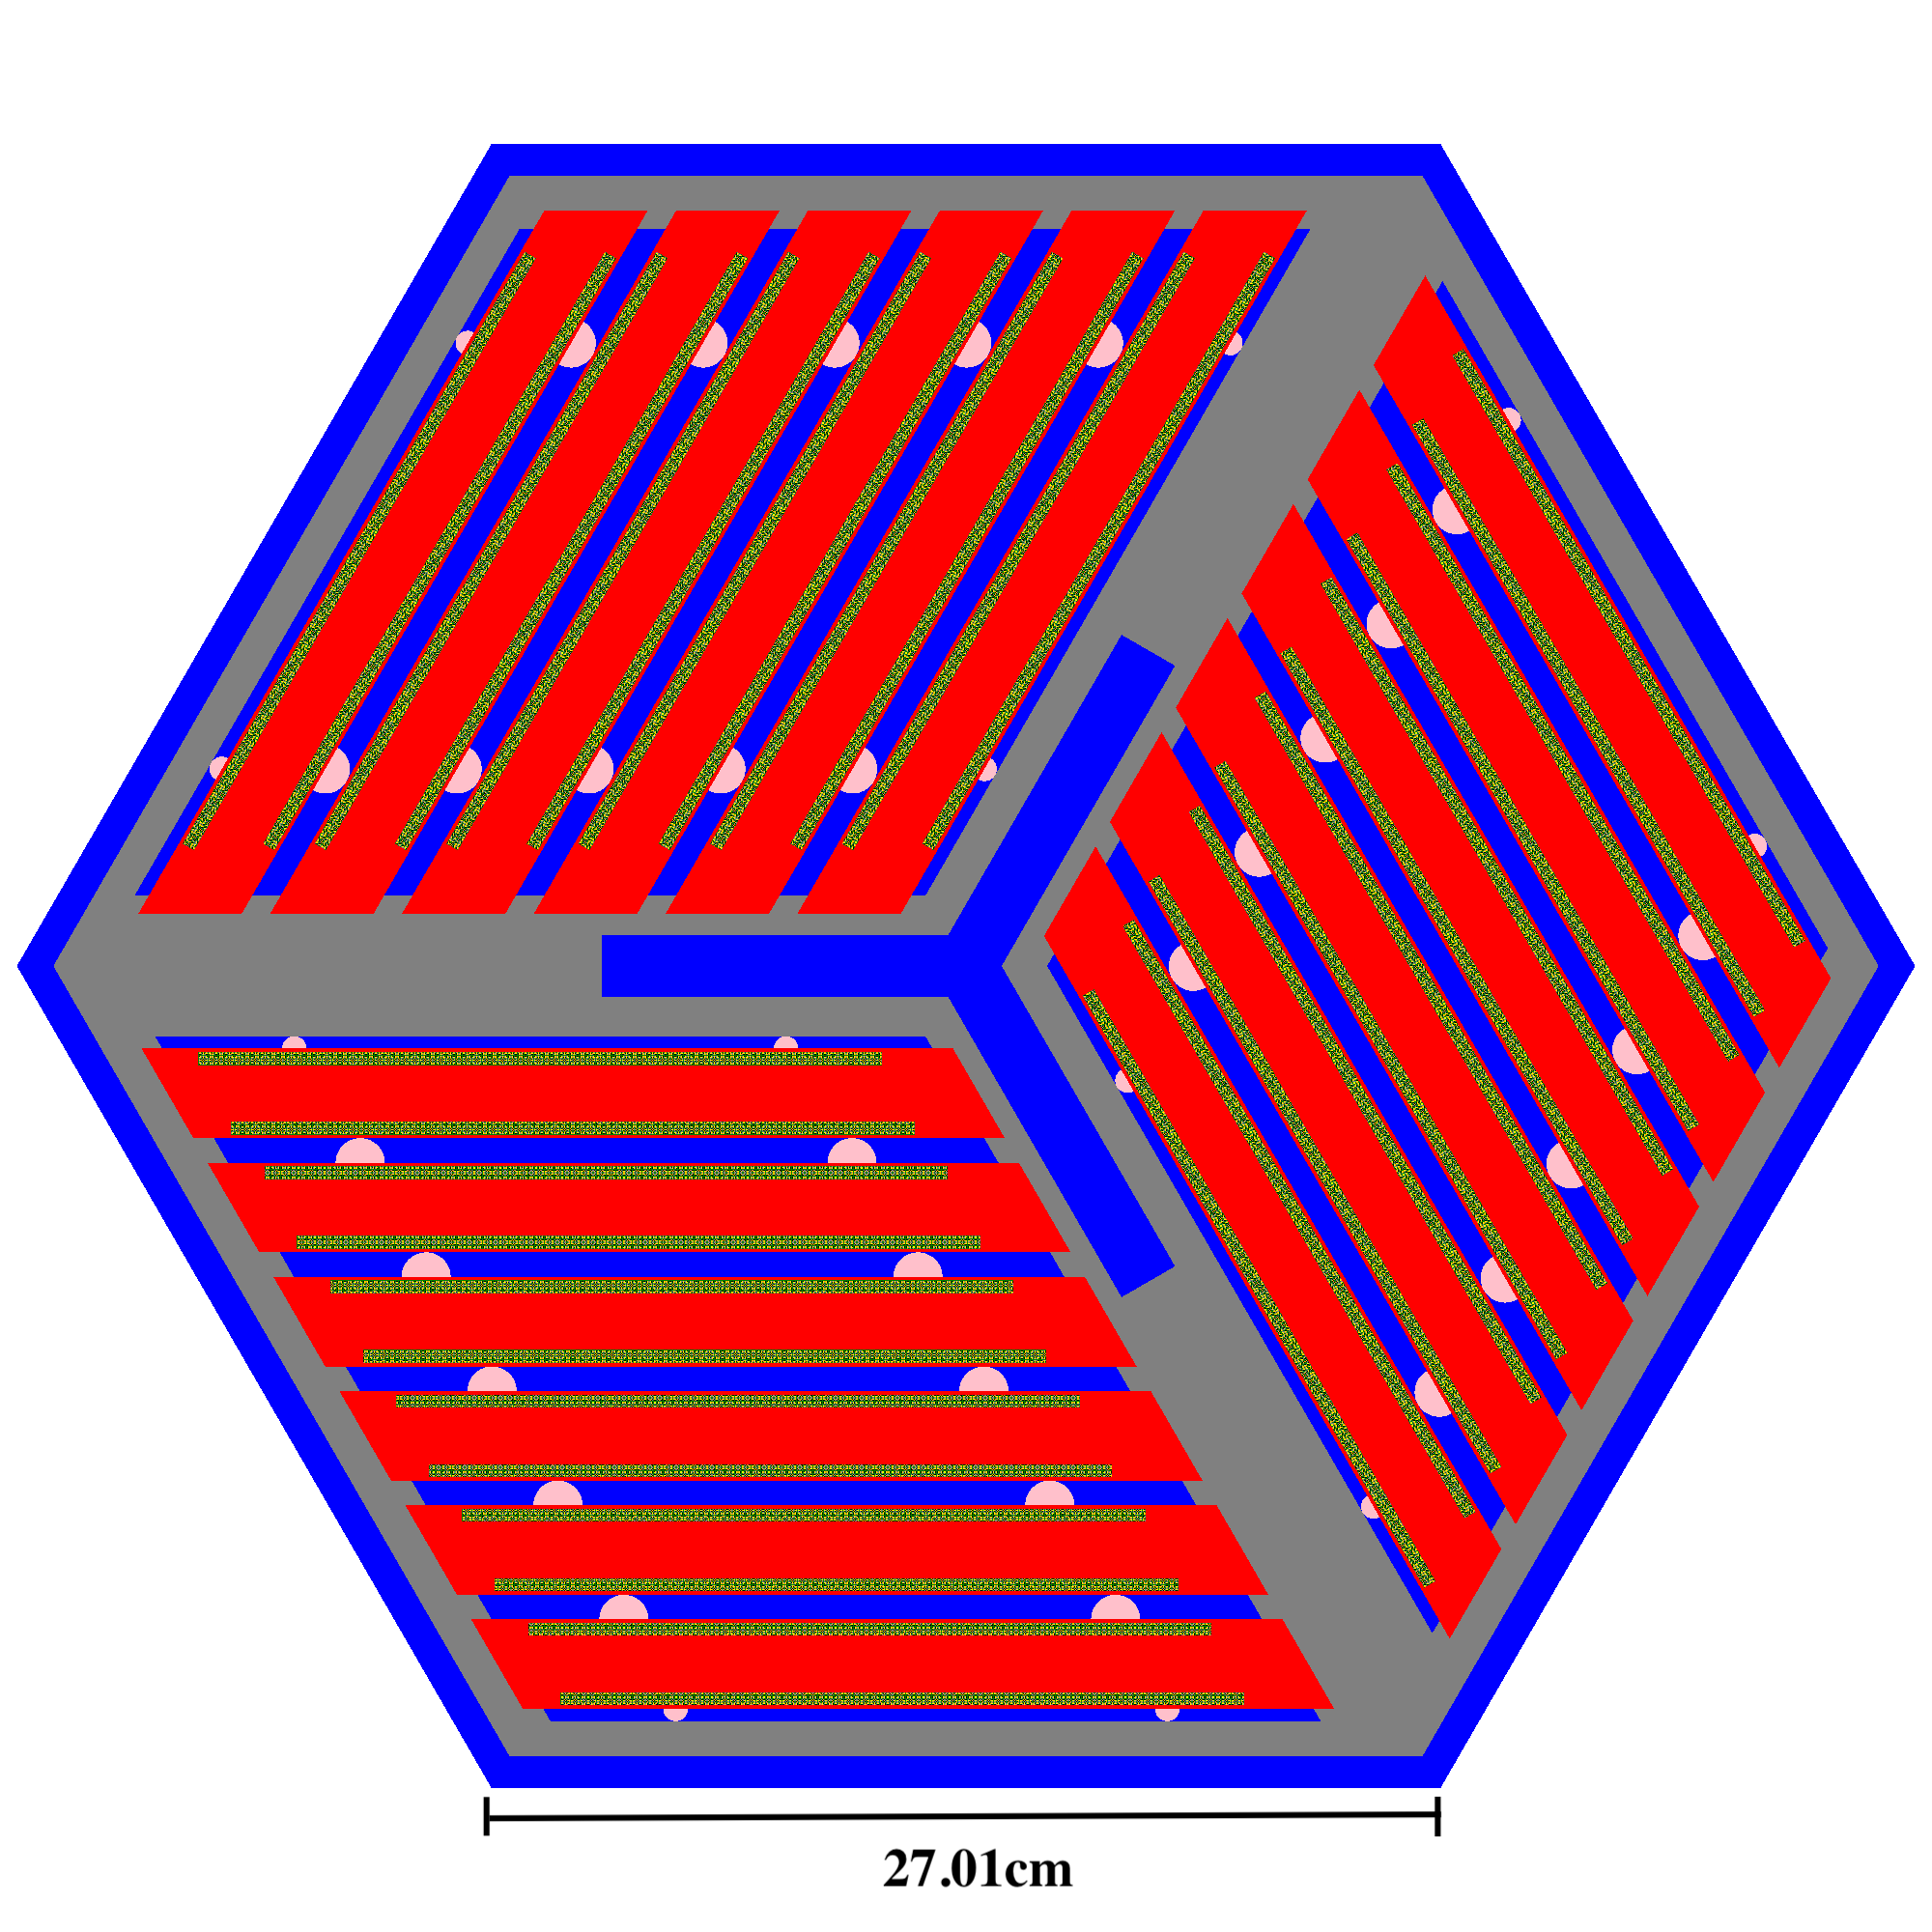
\includegraphics[width=0.27\linewidth]{../docs/figures/ahtr-fuel-element.png} 
        \vspace{-0.2cm}
        \caption{AHTR fuel assembly.}
    \end{figure}
\end{frame}

\begin{frame}
    \frametitle{FHR Benchmark Specifications}
    \begin{itemize}
        \item Only Phase I-A and I-B specifications have been released 
        \item Benchmark participants must produce the following results for 
        the 9 cases: $k_{eff}$, reactivity coefficients ($\beta_{eff}$, 
        $\alpha_D$, $\alpha_{T, FliBe}$, $\alpha_M$), fission source distribution, 
        neutron flux distribution, fuel assembly averaged neutron spectrum
    \end{itemize}
    \vspace{-0.25cm}
    \begin{table}
        \caption{Description of the \acrlong{FHR} benchmark Phase I-A cases 
        \vspace{-0.25cm}
        \cite{noauthor_fluoride_nodate}.}
        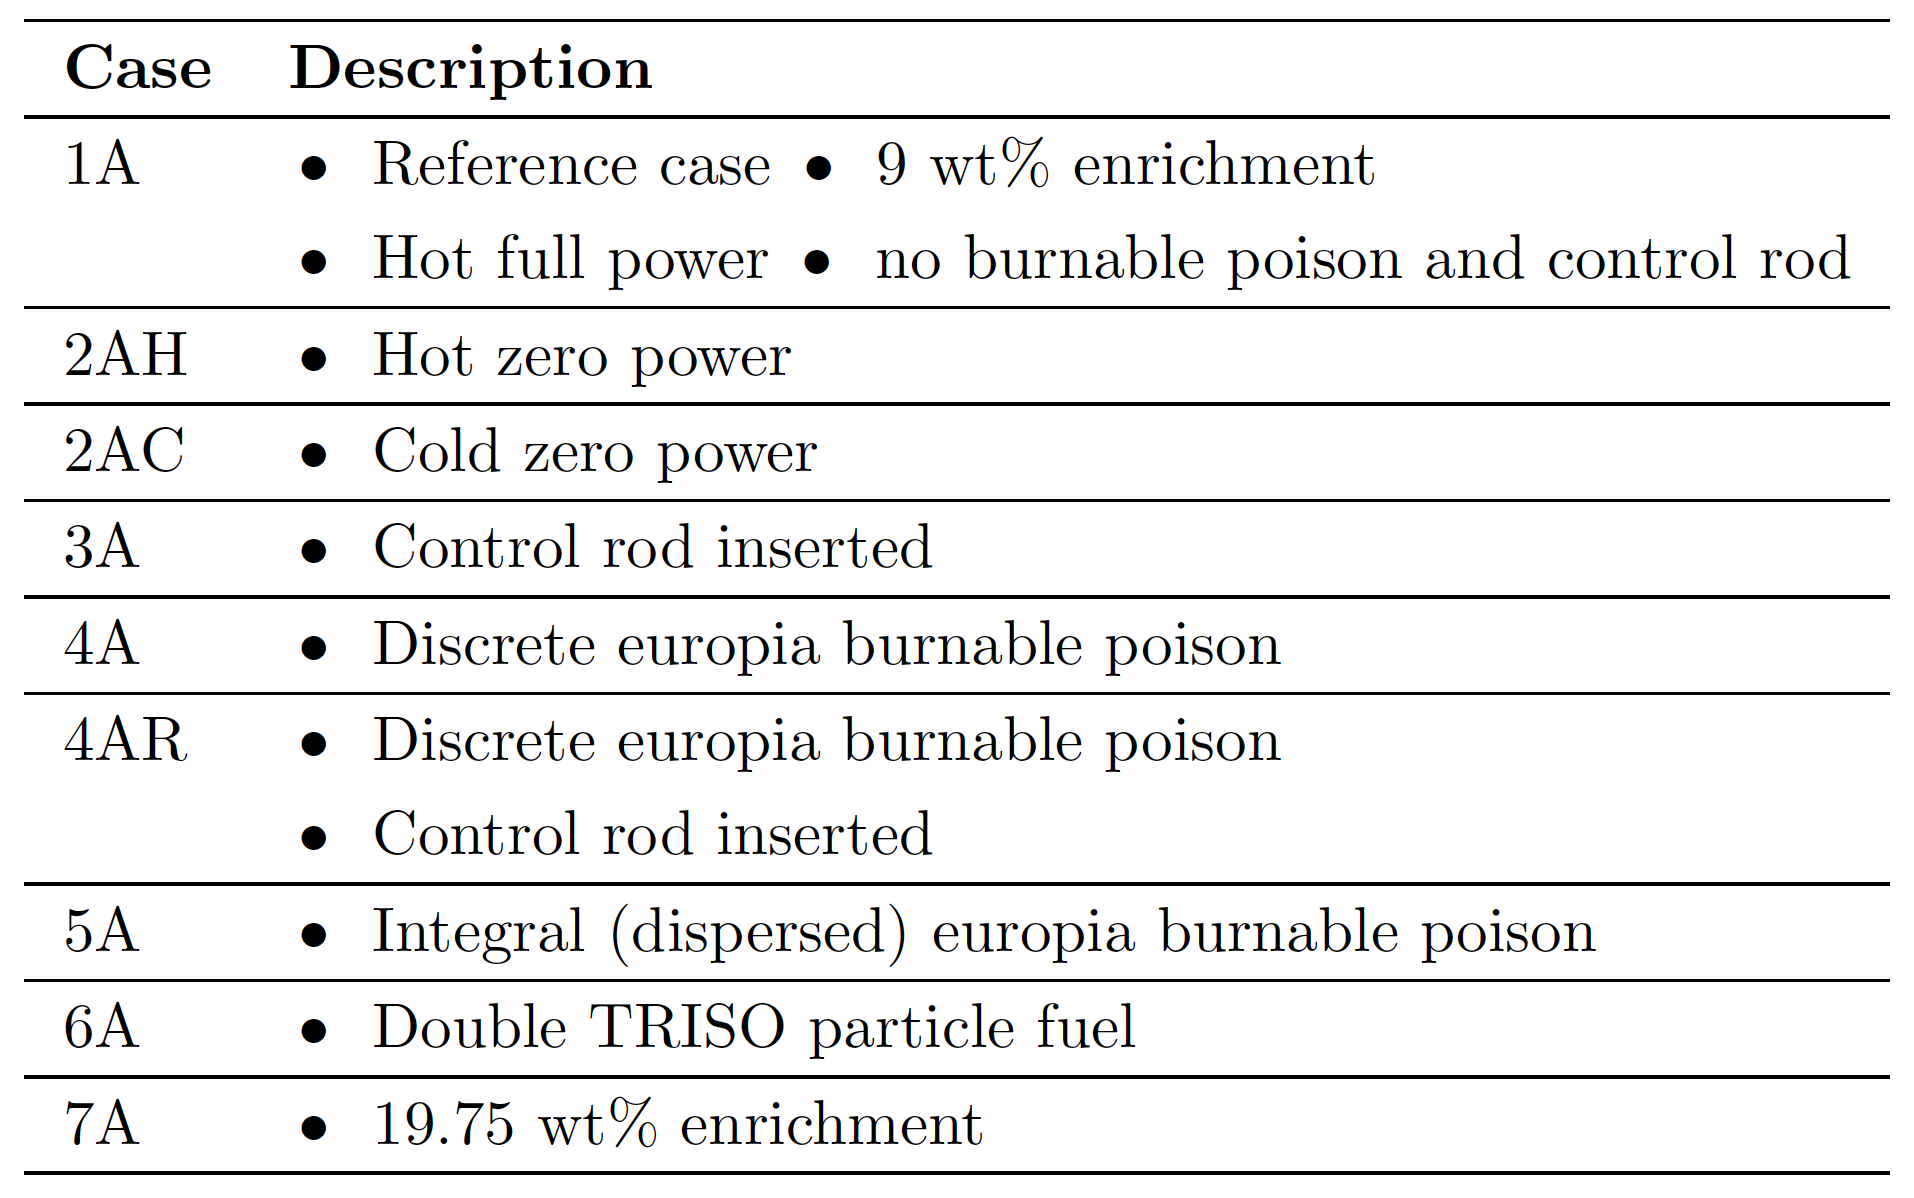
\includegraphics[width=0.6\linewidth]{figures/benchmark-cases.png} 
    \end{table}
\end{frame}

\subsection{FHR Benchmark Results}
\begin{frame}
    \frametitle{FHR Benchmark Phase I-A Results}
    \begin{itemize}
        \item FHR Benchmark Phase I-A: 2D assembly steady state model
        \item In an ANS M$\&$C 2021 conference paper 
        we compared FHR benchmark participants' Phase I-A $k_{eff}$ results.  
        The standard deviation between participants for each case 
        was in the 231 to 514 pcm range, acceptable and notably close given a blind 
        benchmark
    \end{itemize}

    \begin{figure}[]
        \centering
        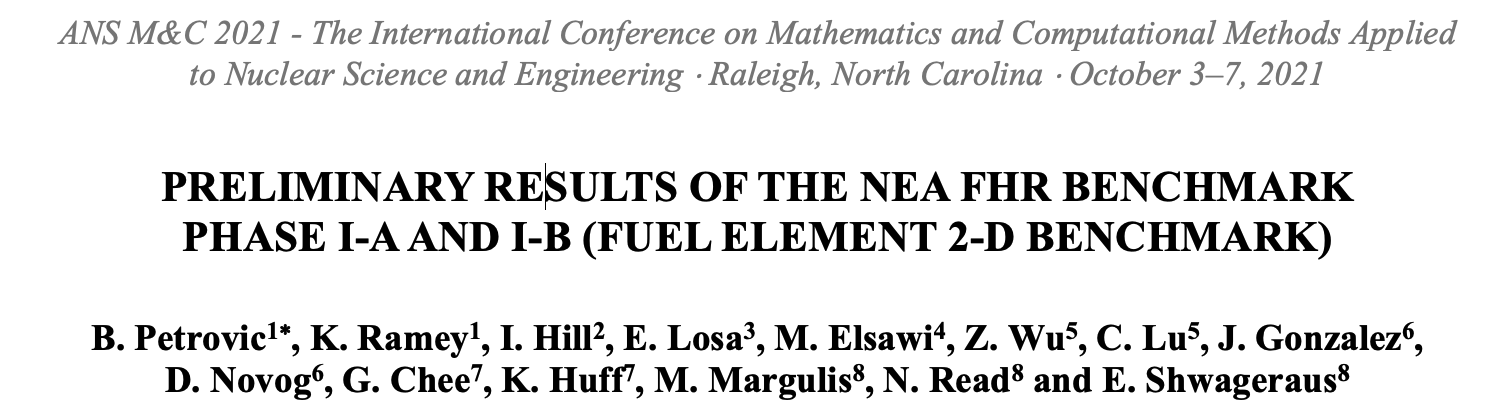
\includegraphics[width=0.85\linewidth]{figures/mnc.png} 
        \caption{FHR benchmark paper presented at M$\&$C 2021 
        \cite{petrovic_preliminary_2021}.}
    \end{figure}
\end{frame}

\begin{frame}
    \frametitle{FHR Benchmark Phase I-A Results}
    \begin{table}
        \caption{UIUC's FHR Benchmark Phase I-A results 
        \cite{chee_arfcfhr-benchmark_2021}.}
        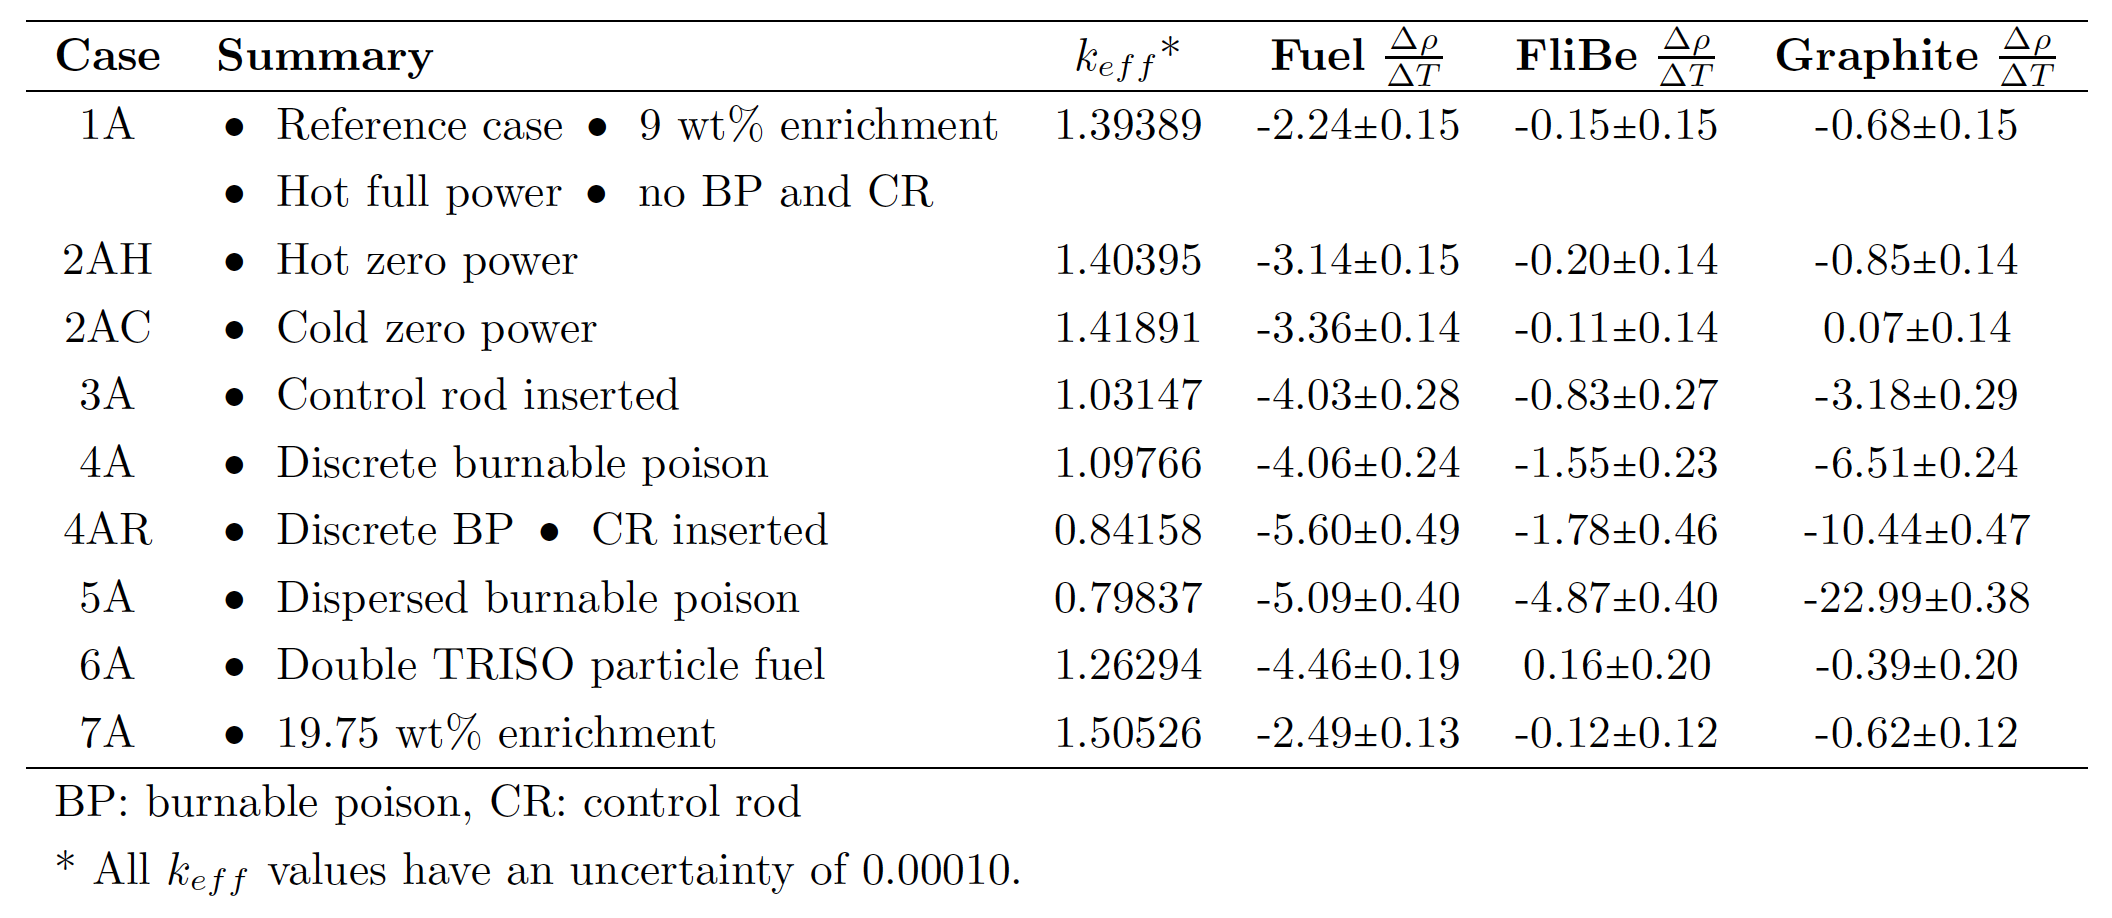
\includegraphics[width=\linewidth]{figures/benchmark-coeff-results.png} 
    \end{table}
    \begin{itemize}
        \item 500 active cycles, 100 inactive cycles, and 200000 neutrons
        \item UIUC's BlueWaters supercomputer with 64 XE nodes
    \end{itemize}
\end{frame}

\begin{frame}
    \frametitle{FHR Benchmark Phase I-A Results}
    \begin{figure}[]
        \centering
        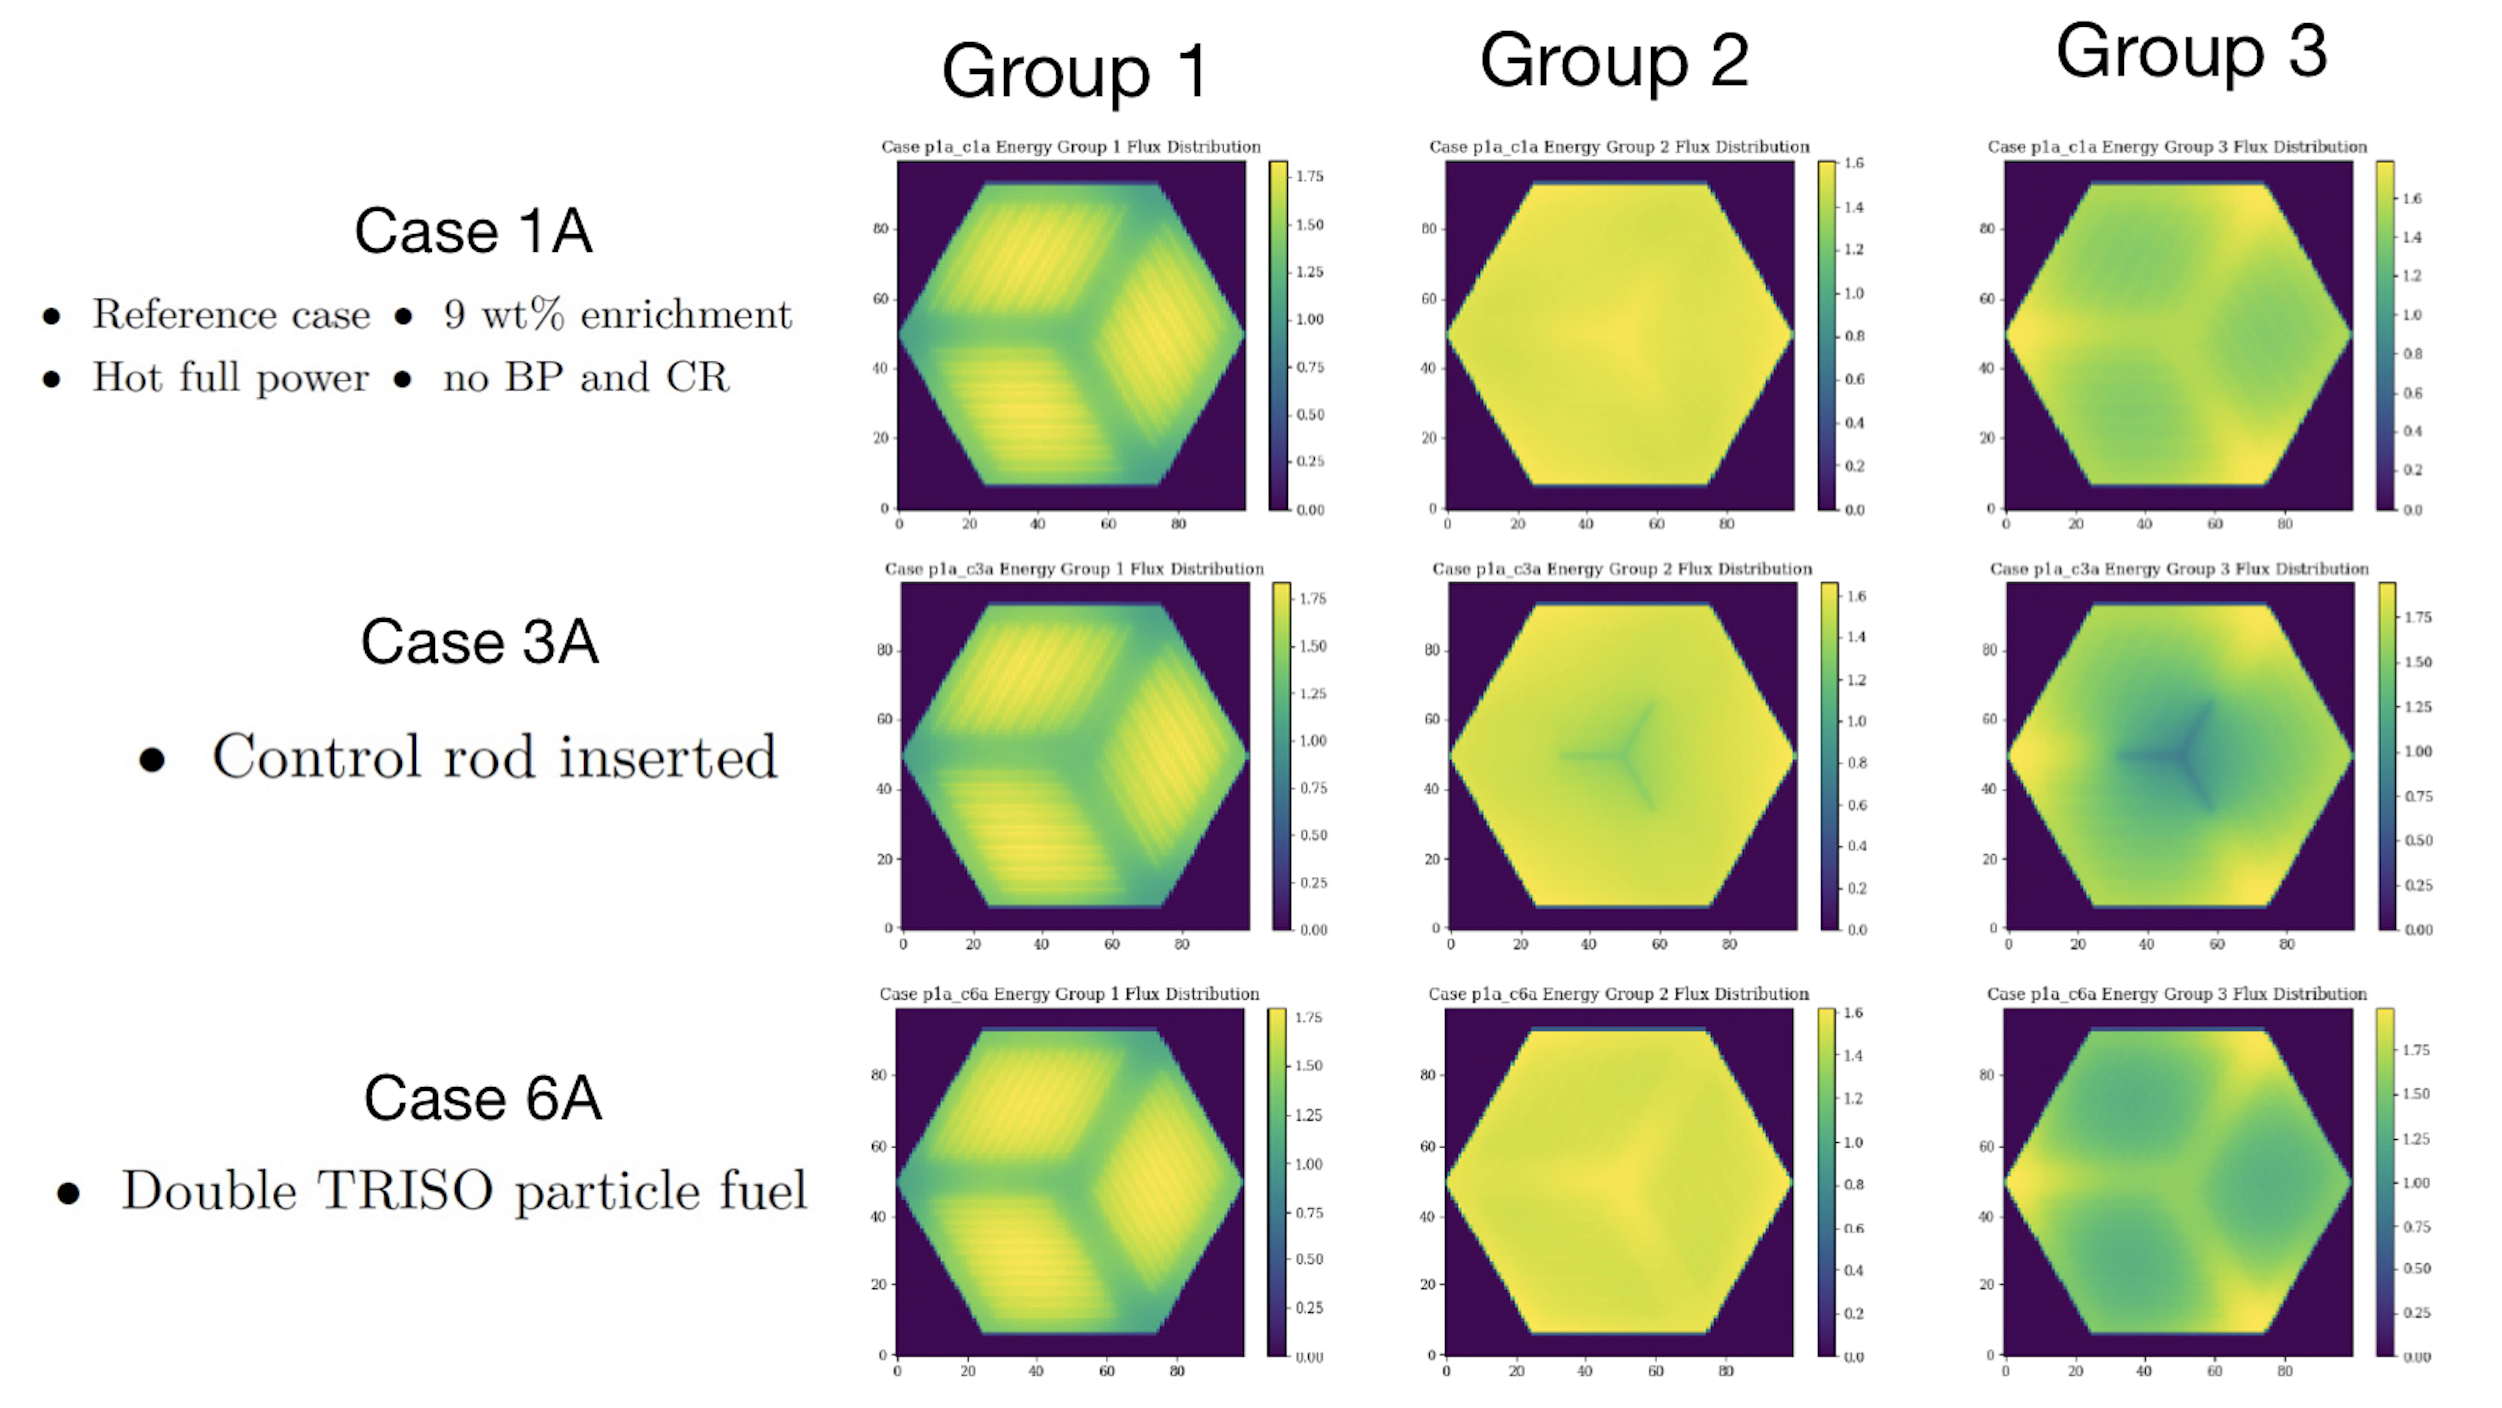
\includegraphics[width=0.9\linewidth]{figures/phase1a-e.png} 
        \vspace{-0.2cm}
        \caption{UIUC results: FHR Benchmark neutron flux 
        distribution in 100 $\times$ 100 mesh for three coarse energy groups: Case 
        1A (above), Case 3A (middle), Case 6A (below). Energy group 1: $E > 0.1$ MeV, 
        Energy group 2: $3 \times 10^{-6} < E < 0.1$ MeV, Energy group 3: $E < 3 \times 10^{-6}$ MeV. }
    \end{figure}
\end{frame}

\begin{frame}
    \frametitle{FHR Benchmark Phase I-B Results}
    \begin{itemize}
        \item FHR Benchmark Phase I-B: 2D assembly depletion model
        \item Benchmark participants are working on resolving differences in 
        these results
    \end{itemize}
    \vspace{-0.2cm}
    \begin{figure}[]
        \centering
        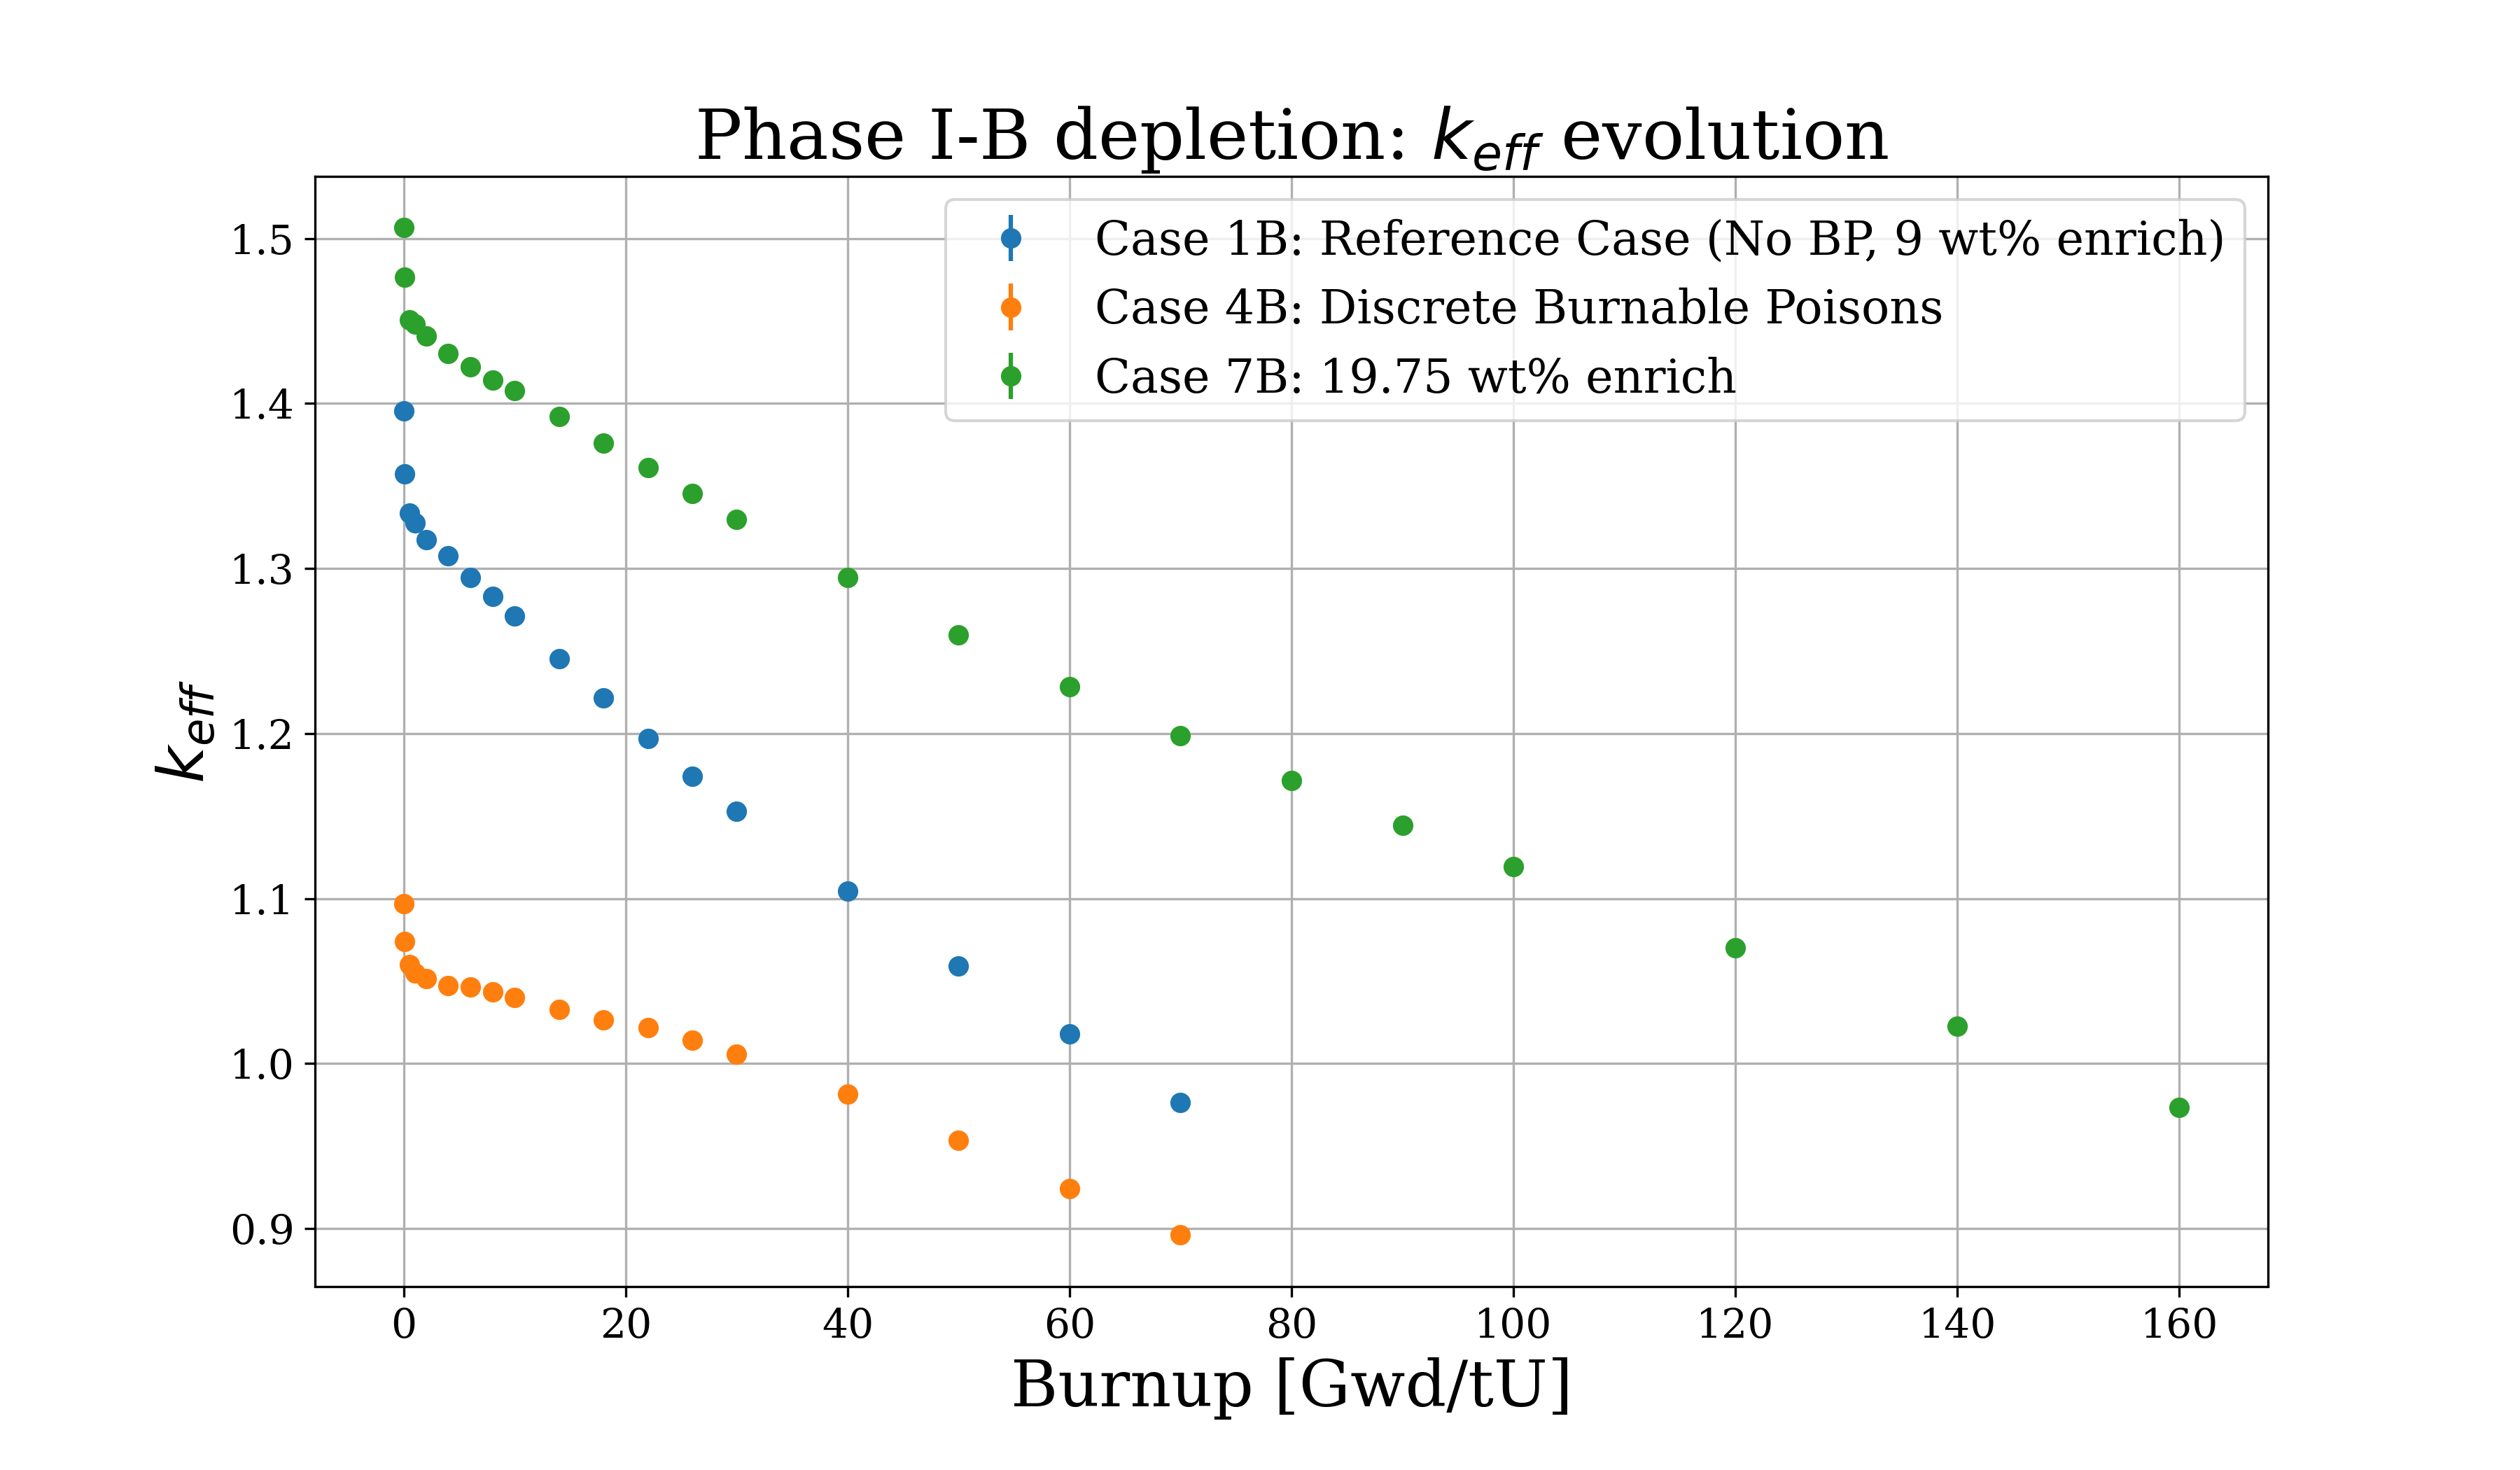
\includegraphics[width=0.75\linewidth]{../docs/figures/phase1b_keff.png} 
        \caption{UIUC results: FHR Benchmark Phase I-B depletion 
        $k_{eff}$ evolution for Cases 1B, 4B, and 7B. Case 1B is the reference case, 
        Case 4B is the discrete \acrlong{BP} case, and Case 7B is the 19.75$\%$ 
        enrichment case. Error bars are included but are barely visible due to the 
        low $\sim$40pcm uncertainty.}
    \end{figure}
\end{frame}

\subsection{AHTR Temperature Model}
\begin{frame}
    \frametitle{AHTR Temperature Model}
    \begin{block}{AHTR Temperature Model}
        \begin{itemize}
            \item I used the open-source MSR simulation tool, Moltres, to conduct AHTR
            full assembly multiphysics simulations 
            \item AHTR Moltres simulations captures thermal feedback effects, absent
            from the purely neutronics OpenMC simulations
            \item I model the steady-state temperature of a 2D x-y AHTR cross-section
        \end{itemize}
    \end{block}
    \begin{block}{Assumptions}
        \begin{itemize}
            \item Conductive heat transfer 
            \item Heat removal by uniform salt flow in coolant regions
        \end{itemize}
    \end{block}

\end{frame}

\subsection{AHTR Temperature Model Results}
\begin{frame}
    \frametitle{AHTR Temperature Model Results}
    \begin{columns}
        \begin{column}{0.6\textwidth}
            \begin{figure}[]
                \centering
                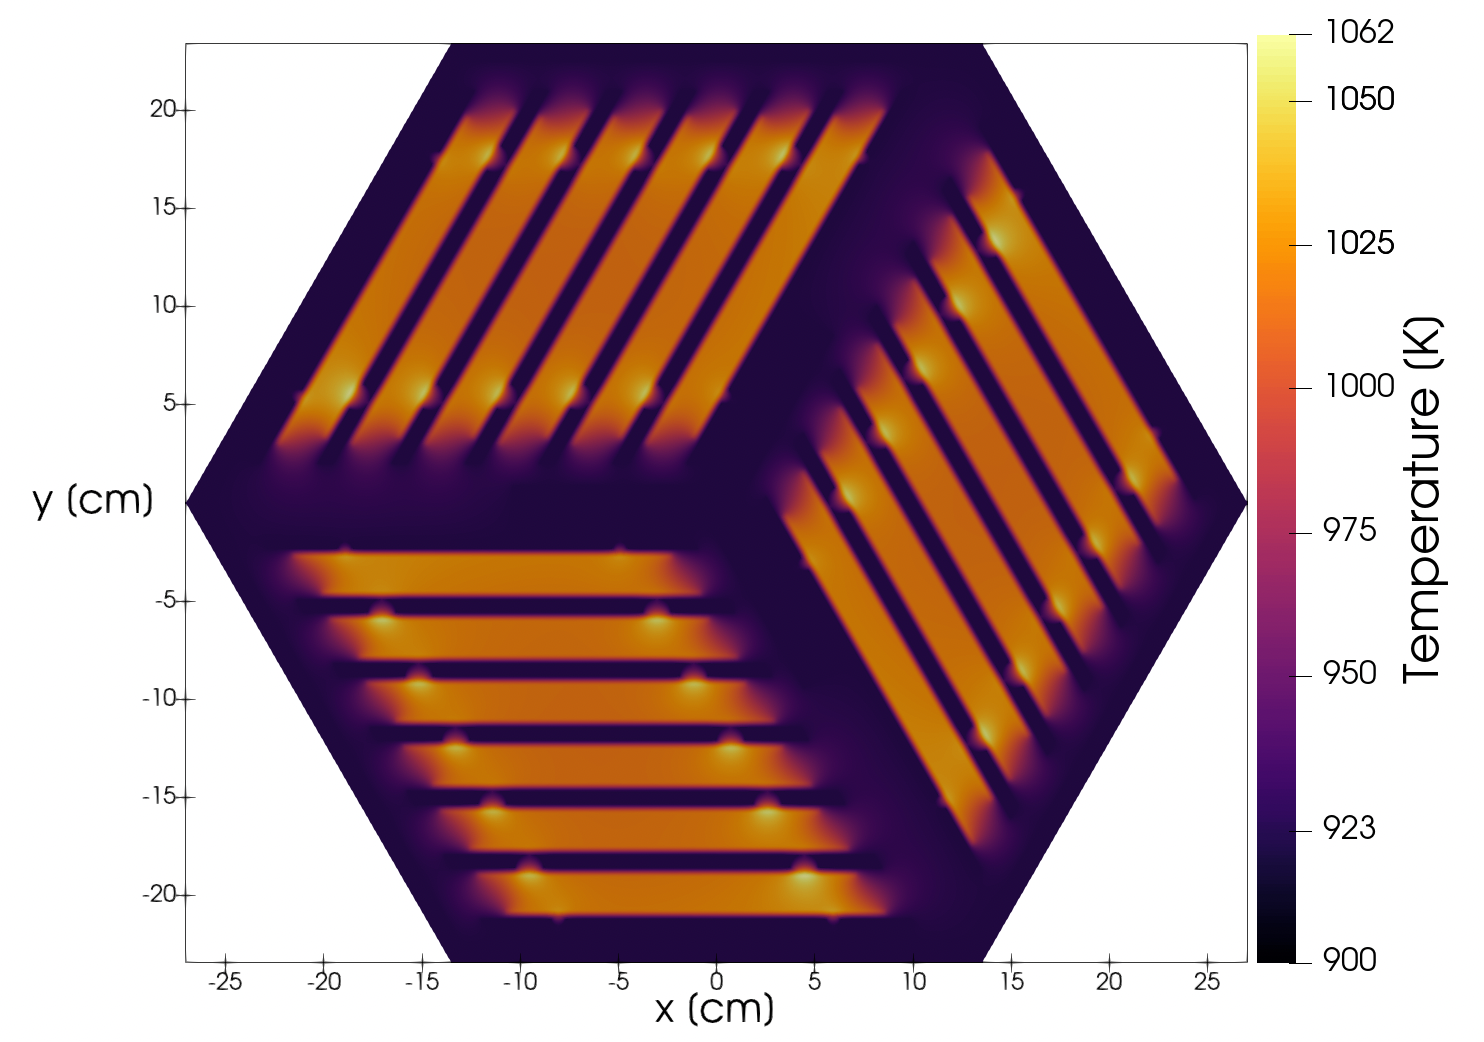
\includegraphics[width=\linewidth]{../docs/figures/benchmark-temperature-model.png} 
                \caption{2D temperature distribution in the \acrfull{AHTR}
                full assembly generated by Moltres.}
            \end{figure}
        \end{column}
        \begin{column}{0.4\textwidth} 
            \begin{block}{Results}
                \begin{itemize}
                    \item Average temperature distribution across the fuel planks are 
                    $\sim 1025K$
                    \item Average temperature of graphite structure is $\sim 935K$
                    \item Temperature peaks at 1062K in the fuel stripes near the spacers
                    \item This could be due to the extra moderation provided by the
                    graphite spacers
                \end{itemize}
            \end{block}
        \end{column}
        \end{columns}
\end{frame}

\subsection{AHTR Model Development: Summary}
\begin{frame}
    \frametitle{AHTR Model Development: Summary}
    \begin{block}{Major Takeaways}
        \begin{itemize}
            \item AHTR has passive safety behavior with negative temperature coeffcients
            \item Increased fuel packing does not always correspond with increased 
            keff due to self-shielding effects 
            \item These results hint at the possibility of minimizing fuel required by 
            optimizing for heterogenous fuel distributions within the core
            \item AHTR temperature peaks in the fuel stripes near the spacers 
        \end{itemize}
    \end{block}
    \begin{block}{I Successfully Completed AHTR Model Development Research Objectives}
        \begin{itemize}
            \item I furthered our understanding of the AHTR design's complexities 
            through neutronics and multiphysics modeling
            \item I participated in the OECD-NEA's FHR Benchmark Phases I-A and I-B
        \end{itemize}
    \end{block}
\end{frame}
